\documentclass{article}
\usepackage[a4paper,margin=1in]{geometry}
\usepackage{titling}
\usepackage{tikz}

\title{Perceptual Interpreter: A Human-Centric Metric for Code Readability}
\author{Tairan Wang \\ Supervisor: Prof. Earl T. Barr}
\date{\today}

\begin{document}

\maketitle

\begin{center}
    \textbf{Internship Proposal} \\
    June 2025 - August 2025
\end{center}

\begin{abstract}
    In software engineering, code readability has long lacked a reliable, cognitively aligned quantitative metric. This research proposes a \textsc{Perceptual Interpreter} based on human short-term memory and abstraction capabilities. The interpreter simulates human code-reading behavior by maintaining a short-term memory model and ultimately providing a readability score. The simulation includes temporally and spatially ordered short-term memory, semantic-based code abstraction, and semantic annotation analysis. Moreover, Large Language Models (LLMs) have demonstrated strong performance in various software engineering tasks, including code generation, comprehension, bug fixing, and test generation. This research leverages LLMs' ability to infer code semantics for abstraction and analysis. Ultimately, we aim to develop a perceptual interpreter aligned with human expert cognition to assess code readability.
\end{abstract}

\section*{Relative Works and Background}
Readable code has better locality and performs better.

\section*{Aims and Objectives}

The early goal of this research is to rapidly develop an interpreter capable of recognizing and parsing explanatory content such as comments. It should include a basic short-term memory simulation and a readability scoring function.

The second phase aims to implement semantic similarity-based memory abstraction and comment analysis to further enhance the interpreter's capabilities.

The third phase focuses on refining the interpreter based on collected human expert feedback. This phase will gradually introduce additional parameters such as human long-term memory, forgetting, and recall mechanisms.

If time permits, after collecting human expert feedback, this research will attempt to train a neural network to weight LLM layer features based on readability scores. Under this weighting, the aggregated LLM layer features will form a new code readability metric, analogous to LPIPS in image similarity assessment.

The minimum expected outcomes of this project are:
\begin{itemize}
    \item A \textsc{Perceptual Interpreter} for a specific programming language, along with its dataset and experimental results, demonstrating its ability to accurately assess the readability of programs written in that language.
    \item A method for constructing or training a \textsc{Perceptual Interpreter} that can be generally applied to any programming language.
    \item A paper submitted to a top-ranked software engineering or machine learning conference.
\end{itemize}

\section*{Work Plan}

\textbf{[Week 1-2]} Develop an interpreter capable of recognizing and parsing explanatory content such as comments. This interpreter should include a basic short-term memory simulation and a readability scoring function. Additionally, develop a refactoring mechanism that can controllably disrupt code structure without affecting program correctness or side effects, thereby altering readability. 

At this stage, short-term memory will allocate a slot when encountering a new variable and release it when the variable goes out of scope or its left-time expires.

\begin{figure}[h!]
    \centering
    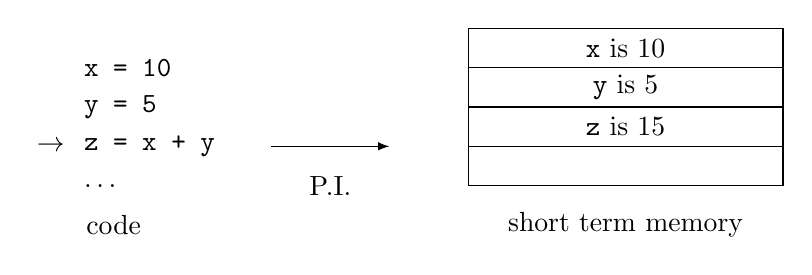
\begin{tikzpicture}[>=latex]
        \node[anchor=west] at (-5,1) {\verb|x = 10|};
        \node[anchor=west] at (-5,0.5) {\verb|y = 5|};
        \node[anchor=west] at (-5,0) {\verb|z = x + y|};
        \node[anchor=west] at (-5,-0.5) {\ldots};
        \node at (-5.3,0) {$\to$};
        \node at (-4.5,-1) {code};

        \draw[->] (-2.5,0) -- (-1,0);
        \node at (-1.75,-0.5) {P.I.};


        \draw (0,1) rectangle (4,1.5);
        \draw (0,0.5) rectangle (4,1);
        \draw (0,0) rectangle (4,0.5);
        \draw (0,-0.5) rectangle (4,0);
        \node at (2,1.25) {\verb|x| is 10};
        \node at (2,0.75) {\verb|y| is 5};
        \node at (2,0.25) {\verb|z| is 15};
        \node at (2,-1) {short term memory};
    \end{tikzpicture}
\end{figure}

\ \\ 
\textbf{[Week 3-4]} Implement memory abstraction based on semantic similarity. Unlike traditional interpreters that retain all environment variables, humans have an abstraction capability. For example, humans abstract functionally coherent code into functions and understand the code by remembering only the function’s purpose rather than its implementation. Similarly, when reading logically coherent code, humans automatically abstract its content, such as "this code performs boundary checks and raises an error" or "this code retrieves user input and validates it."

When similar content exists in short-term memory, humans tend to merge abstractions. Therefore, the \textsc{Perceptual Interpreter} should periodically check for similar memory entries and merge them accordingly. This semantic similarity check can be performed using the embedding space of an LLM or by directly querying it with appropriate prompts.

\begin{figure}[h!]
    \centering
    \begin{tikzpicture}[>=latex]
        \draw (0,1) rectangle (4,1.5);
        \draw (0,0.5) rectangle (4,1);
        \draw (0,0) rectangle (4,0.5);
        \draw (0,-0.5) rectangle (4,0);
        \node at (2,1.25) {\verb|x| is 10};
        \node at (2,0.75) {\verb|y| is 5};
        \node at (2,0.25) {\verb|z| is 15};
        \node at (2,-1) {short term memory};

        \draw (4.25, 1.25) -| (5,0.75);
        \draw[->] (4.25, 0.75) -- (5.75,0.75);
        \draw (4.25, 0.25) -| (5,0.75);

        \draw (6,0.25) rectangle (9.5,1.25);
        \node at (7.75,0.75) {LLM embedding space};

        \draw[->] (7.75, 0.25) --node[fill=white]{if near} (3.5 ,-2);
        \draw (0,-2.5) rectangle (4,-2);
        \draw (0,-3) rectangle (4,-2.5);
        \draw (0,-3.5) rectangle (4,-3);
        \draw (0,-4) rectangle (4,-3.5);
        \node at (2,-2.25) {\verb|x| is 10, \verb|y| is 5, \verb|z| is 15};
        \node at (2,-4.5) {update memory};

        \draw[->] (7.75, 0.25) --node[fill=white]{if not} (7.75 ,-3
        \node at (7.75, -3.25) {no change in memory};
    \end{tikzpicture}
    \caption{Demo}
\end{figure}

\ \\ 
\textbf{[Week 5-6]}

\ \\
\textbf{[Week 7]}

\ \\
\textbf{[Week 8]}


\end{document}
